\subsection*{Monte Carlo Sampling}

% Week 8

\begin{defe}[Empirical distribution] \label{defe: em_dist}
    Let $x_1 , \ldots , x_n$ be an iid real-valued sample from a cdf $F$. The function
    \begin{equation*}
        F_{n} (x) = \frac{1}{N} \sum_{i=1}^{N} \Id_{\left\{ x_i \leq x \right\}} (x) , \quad x \in \RR
    \end{equation*}
    is called the {\bf empirical cdf} of the data \cite{KroeseDirkP2013SMaC}*{page 196}.
\end{defe}

\begin{figure}[ht]
    \centering
    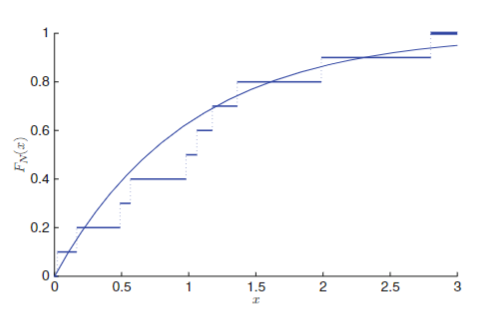
\includegraphics[scale=1.0]{img/bay_inf/emp_cdf_exp_1.png}
    \caption{The empirical cdf \ref{defe: em_dist} for a sample size $10$ from a $\Exp (0.2)$ distribution as well as the true cdf. Image from \cite{KroeseDirkP2013SMaC}*{page 197}.}
    \label{fig: emp_cdf_exp_1}
\end{figure}

Note that for the ordered sample $x_{(1)} < x_{(2)} < \cdots < x_{(N)}$,

\begin{equation*}
    F_{N} \left( x_{(i)} \right) = \frac{i}{N}.
\end{equation*}

assuming for the sake of simplicity that all $\left\{ x_i \right\}$ take on different values. If instead of deterministic $\left\{ x_i \right\}$ we take random $X_i$, then $F_N (x)$ becomes random as well. To distinguish between the deterministic and the random case, let us denote the random empirical cdf by $\hat{F}_{N} (x)$. We now have
\begin{equation*}
    \PP \left[ \hat{F}_{N} (x) = \frac{i}{N} \right] = \PP \left[ X_{(i)} \leq x , X_{(i+1)}  x \right] = \binom{N}{i} \left( F(x) \right)^{i} \left( 1 - F(x) \right)^{N-i}
\end{equation*}
\cite{KroeseDirkP2013SMaC}*{page 198}. The above equation can be summarized as $N \hat{F}_{N} (x) \sim \Bin (N, F(x))$. Consequently,
\begin{align*}
    \EE \left[ \hat{F}_{N} (x) \right]  & = F(x)                          \\
    \Var \left[ \hat{F}_{N} (x) \right] & = F(x) \left( 1 - F(x) \right).
\end{align*}
Moreover, by the law of large numbers and the central limit theorem, we have
\begin{equation*}
    \PP \left[ \lim_{N \to \infty} \hat{F}_{N} (x) = F (x) \right] = 1,
\end{equation*}
and
\begin{equation*}
    \lim_{N \to \infty} \PP \left[ \frac{\hat{F}_{N} (x) - F(x)}{\sqrt{F(x)(1-F(x)/N)}} \right] = \Phi (z).
\end{equation*}

\begin{defe}[Confidence Intervals] \label{defe: confd_int}
    Let $X_1 , \ldots , X_n$ be random variables with a joint distribution depdending on a parameter $\theta \in \Theta$. Let $T_1 < T_2$ be functions of the data but not of $\theta$. The random interval $(T_1 , T_2)$ is called a {\bf stochastic confidence interval} for $\theta$ with confidence $1 - \alpha$ if
    \begin{equation*}
        \PP_{\theta} \left[ T_1 < \theta < T_2 \right] \geq 1 - \alpha \quad \text{for all} \quad \theta \in \Theta.
    \end{equation*}
    If $t_1$ and $t_2$ are the observed values of $T_1$ and $T_2$, then the interval $(t_1 , t_2)$ is called the {\bf numerical confidence interval} for $\theta$ with confidence $1 - \alpha$ \cite{KroeseDirkP2013SMaC}*{page 128}.
\end{defe}

An approximate $1 - \alpha$ confidence interval for $F(x)$ is
\begin{equation*}
    F_N (x) \pm z_{1 - \alpha / 2} \sqrt{\frac{F_N (x) (1 - F_N (x))}{N}}
\end{equation*}
where $z_{1 - \alpha / 2}$ is the $1 - \alpha / 2$ quantile of the standard normal distribution. Moreover for the ordered sample $x_{(1)} < x_{(2)} < \cdots < x_{(N)}$, an approximate $1 - \alpha$ confidence interval for $F(x_{(i)})$ is
\begin{equation*}
    \frac{i}{N} \pm z_{1 - \alpha / 2} \sqrt{\frac{i(1 - i/n)}{N^2}}
\end{equation*}
\cite{KroeseDirkP2013SMaC}*{page 198}.